\chapter{The Forward Model}
\label{ch:formodel}

In this chapter, we present the forward model to which we apply all our methodology. We follow the Michelson interferometer for passive atmospheric sounding (MIPAS) handbook~\cite{mipas2000handbook} and simulate data according to an idealised cloud-free atmosphere in local thermodynamic equilibrium, assuming a measurement instrument with infinite spectral resolution and no pointing errors.
This is a simplified forward model and we do not include any other instrument-specific details, such as sensor area or antenna response, as they are not available to us. 
\begin{figure}[ht!]
	\centering
	\input{LIMB.pdf_tex}
	\caption[Schematic of measurement and analysis geometry.]{Schematic of measurement and analysis geometry, not to scale.
		The stationary satellite, at a constant height $h_\text{sat}$ above Earth, takes $m$ measurements along its line-of-sight defined by the line $\Gamma_j$.
		Each measurement has a limb height $\ell_j$, $j=1,2,\dots,m$ defined as the closest distance of $\Gamma_j$ to the Earth's surface.
		Between $h_{L,0} \approx 7$km and $h_{L,n} \approx 83$km, the atmosphere is discretised into $n$ layers as illustrated by the solid green lines.}
	\label{fig:LIMB}
\end{figure}


A satellite at a constant height $h_{\text{sat}}$ points through the atmosphere (limb-sounding) and measures thermal radiation of gas molecules along its straight line of sight $\Gamma_j$, see  Figure~\ref{fig:LIMB}.
One measurement of the thermal radiation of one specific molecule, in our case ozone, denoted by the ozone volume mixing ratio (VMR) $x(r)$ at distance $r$ from the satellite, at the wave number $\nu$, is given by the path integral
\begin{align}
	\label{eq:RTE} 
	y_j =   \int_{\Gamma_j}  B(\nu,T) k(\nu, T)   \frac{p(T)}{k_{\text{B}} T(r)}  x(r)  \tau(r) \text{d}r + \eta_j \, \\
	\tau(r) = \exp{ \Bigl\{ - \int^{r}_{r_\text{obs}}  k(\nu, T)   \frac{p(T)}{k_B T(r^{\prime})}  x(r^{\prime}) \text{d}r^{\prime} \Bigr\} } \, ,\label{eq:absRTE} 
\end{align}
which is the radiative transfer equation (RTE)~\cite{mipas2000handbook}.
For more information on the processes within the atmosphere for ozone, we refer to~\cite{Lee2020NightOzone}.
We define a tangent height $h_{\ell_j}$ and $\Gamma_j$ for each $j=1,2,\ldots,m$, so that the data vector $\bm{y} \in \mathbb{R}^m$ including some additive noise $\eta_j$.
Within the atmosphere, the number density $p(T) / (k_{\text{B}} T(r))$ of molecules is dependent on the pressure $p(T)$, the temperature $T(r)$, and the Boltzmann constant $k_{\text{B}}$.
The factor $\tau(r)\leq 1$ accounts for re-absorption of the radiation along the line-of-sight, which makes the RTE non-linear.
The absorption constant
\begin{align}
	k(\nu, T) = L(\nu, T_{\text{ref}}) \frac{Q(T_{\text{ref}})}{Q(T)} \frac{ \exp{\{ - c_2 E^{\prime \prime} / T\}} }{\exp{\{ - c_2 E^{\prime \prime} / T_{\text{ref}} \}}} \frac{ 1- \exp{\{ - c_2 \nu  / T \}} }{1 - \exp{\{ - c_2 \nu / T_{\text{ref}} \}}}
\end{align}
is dependent on the line intensity $L(\nu, T_{\text{ref}})$ at reference temperature $T_{\text{ref}} =296K $, the lower-state energy $ E^{\prime \prime} $ in $\text{cm}^{-1}$ of the targeted transition and the second radiation constant $c_2\coloneqq hc/k_{\text{B}} \approx 1.44\text{cmK}$ as in the HITRAN database \cite{gordon2022hitran2020}, with Planck's constant $h$ and speed of light $c$.
Since we assume that the measurement device has a negligible frequency window, we neglect line broadening around $\nu$ for the calculations of $L(\nu, T_{\text{ref}})$, which would normally be modelled as a convolution of the normalised Lorentz profile (collisional/pressure broadening) and the normalised Doppler (thermal broadening) profile~\cite{mipas2000handbook}.
Additionally, we target one specific molecule and calculate $k(\nu, T)$ accordingly, which usually would involve summing the individual absorption constants for multiple radiating molecules weighted by their respective VMR~\cite{mipas2000handbook}.
The total internal partition function is given as:
\begin{align}
	Q(T )= g^{ \prime} \exp{\{ - \frac{ c_2 E^{ \prime} }{T}\}} + g^{\prime \prime} \exp{\{ - \frac{ c_2 E^{\prime \prime} }{T}\}} \, ,
\end{align}
with the statistical weight $ g^{\prime \prime}$ for the lower and $ g^{ \prime}$ for the upper energy state (also called the degeneracy factors) accounting for the molecule's non-rotational and rotational energy states (see~\cite{vsimevckova2006einstein}), and the upper state energy $E^{ \prime} = E^{ \prime\prime} + \nu$.
Under the assumption of local thermodynamic equilibrium (LTE), the black body radiation acts as a source function
\begin{align}
	B(\nu,T)   = \frac{2 h c^2 \nu^3}{\exp{\{\frac{c_2\nu}{ T}\}}-1}\, .
\end{align}

For fundamentals on the RTE, we recommend~\cite[Chapter 1]{rybicki2000rte}, and for a more comprehensive model, we refer to \cite{read2006forwardModel}.

To calculate the integrals in Eq.~\ref{eq:RTE} and Eq.~\ref{eq:absRTE} numerically, we discretise the atmosphere in $n$ layers, where the $i-th$ layer is defined by two spheres of radii $h_{L,i-1} < h_{L,i}$, for $i = 1, \dots, n$, with $h_{L,0}$ and $h_{L,n} $.
Then the ozone VMR $\bm{x} =\{x_1,x_2,\ldots,x_n\} \in \mathbb{R}^{n}$, pressure $\bm{p} =\{p_1,p_2,\ldots,p_n\} \in \mathbb{R}^{n}$ and temperature $\bm{T} =\{T_1,T_2,\ldots,T_n\} \in \mathbb{R}^{n}$, as well as all other height dependent parameters, are discretised profiles with constant values in between the heights $h_{L,i-1}$ and $h_{L,i}$.
Above $h_{L, n}$ and below $h_{L,0} $, the ozone VMR is set to zero, so no signal can be obtained.
We evaluate the integral in Eq.~\eqref{eq:RTE} for one noise-free measurement $\bm{A_{j}}(\bm{p},\bm{T},\bm{x})$, using the trapezoidal rule.
Here, each entry of $\bm{A}(\bm{p},\bm{T},\bm{x})\in \mathbb{R}^{m}$ includes multiple evaluations of the integral in Eq.~\ref{eq:absRTE} to calculate the absorption $\tau(r)$.
%Note that, since we aim to provide estimates over pressure $\bm{p}$ and temperature $\bm{T}$, we explicitly include them as parameters in our forward model.
The data vector
\begin{align}
	\bm{y} = \bm{A}(\bm{x}) + \bm{\eta}\, 
\end{align}
includes an additive noise vector $\bm{\eta} \in \mathbb{R}^{m}$, where we define the non-linear forward model as $\bm{A}(\bm{x}) \coloneqq \bm{A}(\bm{x},  \bm{p},\bm{T})   \in \mathbb{R}^{m}$ for brevity.
Similarly, we define $\bm{A}_L$, which denotes the linear forward model matrix and neglects absorption (e.g. set $\tau = 1$ in Eq.~\eqref{eq:absRTE}) and enables matrix-vector multiplication $\bm{A}_L \bm{x}$ to compute noise-free linear data.

Further, we classify the inverse problem as a weakly non-linear inverse problem, because neglecting the absorption changes the measurements only slightly (about $1\%$, see Sec.~\ref{sec:affineMap}).

\section{Singular Value Decomposition of the Forward Model}
\textcolor{red}{understanding the forward map}
\label{sec:SVD}
Before simulating some data, we provide a quick and intuitive way of assessing if the data collection is effective, how much information is passed through the forward model, and how the signal-to-noise ratio (SNR) and the measurement strategy affects that information.
One way of doing this is via a singular value decomposition (SVD) of the forward model matrix
\begin{align}
	\bm{A}_L = \sum_{i =1}^{r} \bm{u}_i  \sigma_i \bm{v}^T_i = \bm{U} \bm{\Sigma} \bm{V}^T
\end{align}
where $r = \min\{m,n\}$ for a forward model matrix $\bm{A}_L \in \mathbb{R}^{m \times n}$.
Consider noise-free measurements $\bm{A}_L\bm{x}$ for a satellite at a fixed height of $h_{\text{sat}} = 500$km above sea level.
Our main objective is to measure ozone $\bm{x}$, so our forward model $\bm{A}_L$ includes temperature and pressure, the latter is dominant, see Fig.~\ref{fig:PriorPressOverTemp}, decreases exponentially in height and hence does affect the information passed through the model.
If the pressure is high, the signal is large.
If the pressure is low, the signal is low and the data is noise-dominated.

The SVD gives us information on how information is picked up from the parameter space by the forward model, described through the right singular values $\bm{v}_i$.
The singular values $\sigma_i $, ordered in size from the largest $\sigma_1$ to the smallest $\sigma_{r}$, weigh that information from the right singular values to the left singular values $\bm{u}_i$, which project onto the data space.
For a large singular value, we can say that the forward model is informative about parameter structures according to the corresponding right singular vector and vice versa. \textcolor{red}{WQhat is the vice versa? Not clear what you are saying. }
%Note that we obtain the same results using the non-linear forward model $\bm{A}(\bm{x})$ to do this analysis, where we would rewrite to the matrix-vector multiplication $\bm{A}_{NL} \bm{x}$, where $\bm{A}_{NL}$ is depend on $\bm{x}$.
Further, for very small singular values $\sigma_i \ll \sigma_1/\text{SNR}$ below the RMS noise level or the noise standard deviation (STD), we can introduce an effective rank $r_{\text{eff}} \leq r$.
Then, the parameter space spanned by $ \{\bm{v}_{r_{\text{eff}} +1}, \dots ,\bm{v}_r \}$ is noise-dominated in the corresponding data space, see Figure \ref{fig:nullSpace}.
This is based on the rough assumption that if we define the SNR as \textcolor{red}{don't put citations in equations -- it's very weird.}
\begin{align}
	\text{SNR} \coloneqq \frac{\max(y)}{\text{STD noise}} = \frac{\text{peak signal}}{\text{RMS noise}} \text{\cite{fox2025BlokkLecNot}} \label{eq:SNR} \, ,
\end{align}
then the maximum singular value $\max(y) \approx \sigma_1$ and the information transmitted through the forward model corresponds roughly to the singular values $\sigma_i \gtrsim \max(y)/ \text{SNR}$.
See~\cite{tan2016LecNot} for a more comprehensive analysis.

\textcolor{red}{why is this plot here before you defined the cases? That's not remotely OK.}
\begin{figure}[ht!]
	\centering
	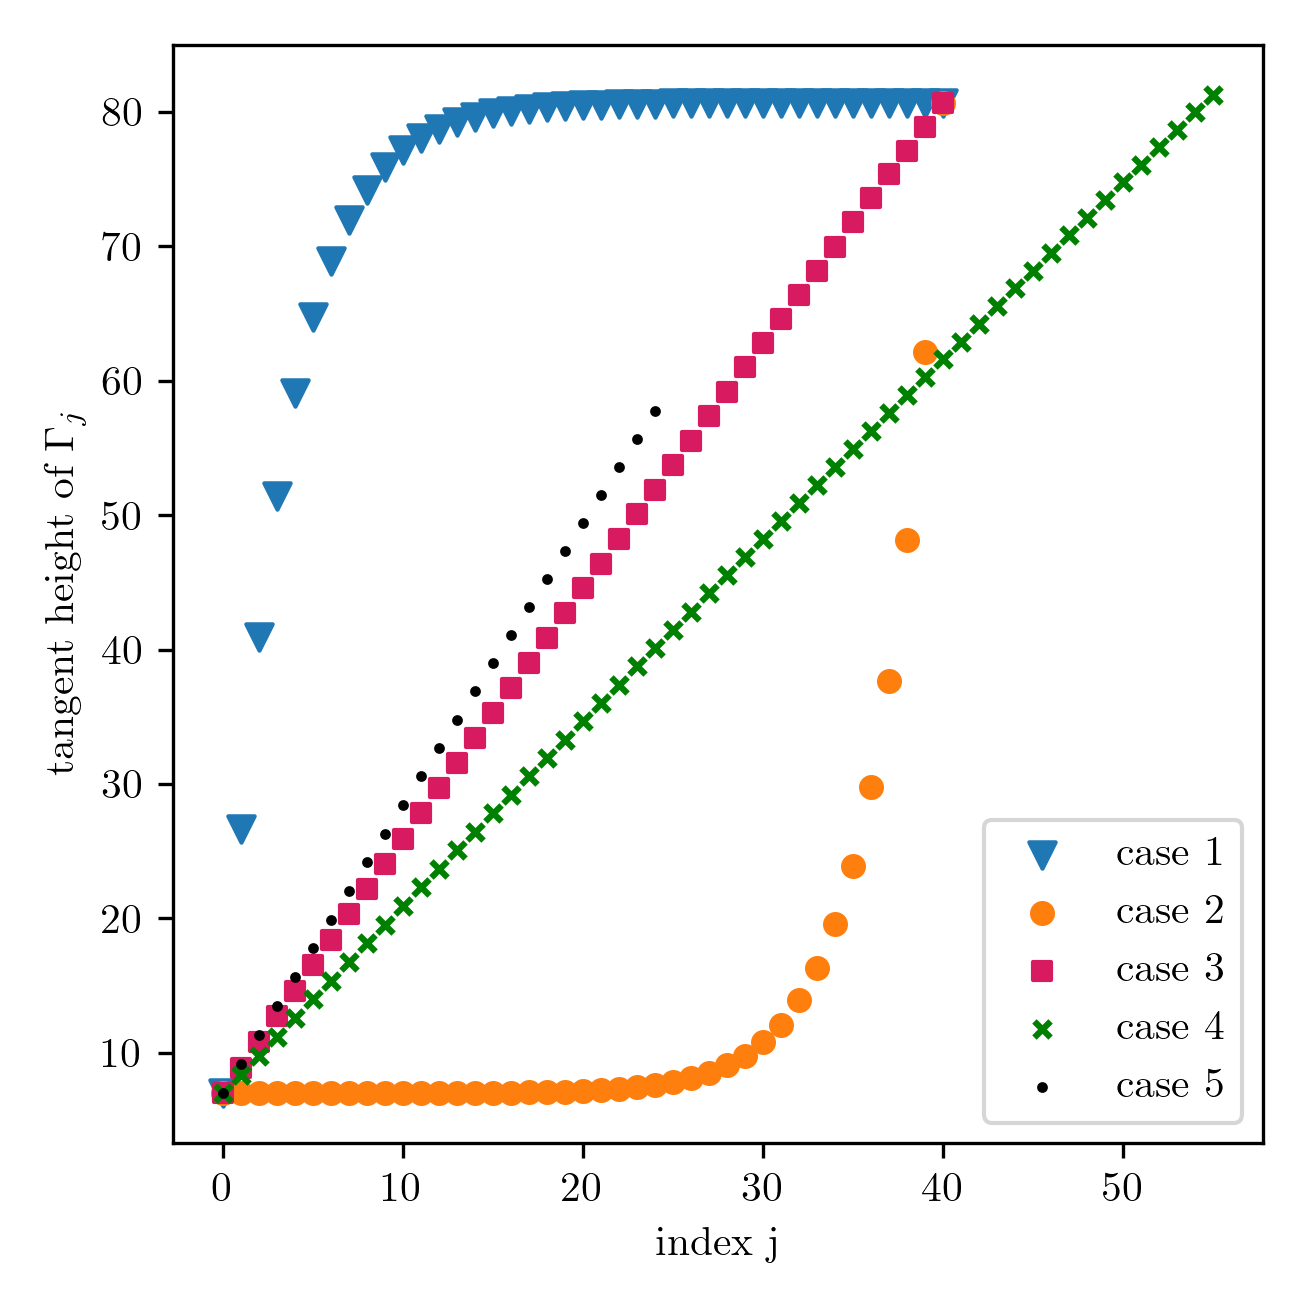
\includegraphics{MeasTangHeight.png}
	\caption[Tangent heights for different sequences of measurements.]{Tangent heights for five different sequences of measurements.}
	\label{fig:TangHCases}
\end{figure}
\begin{figure}[ht!]
	\centering
	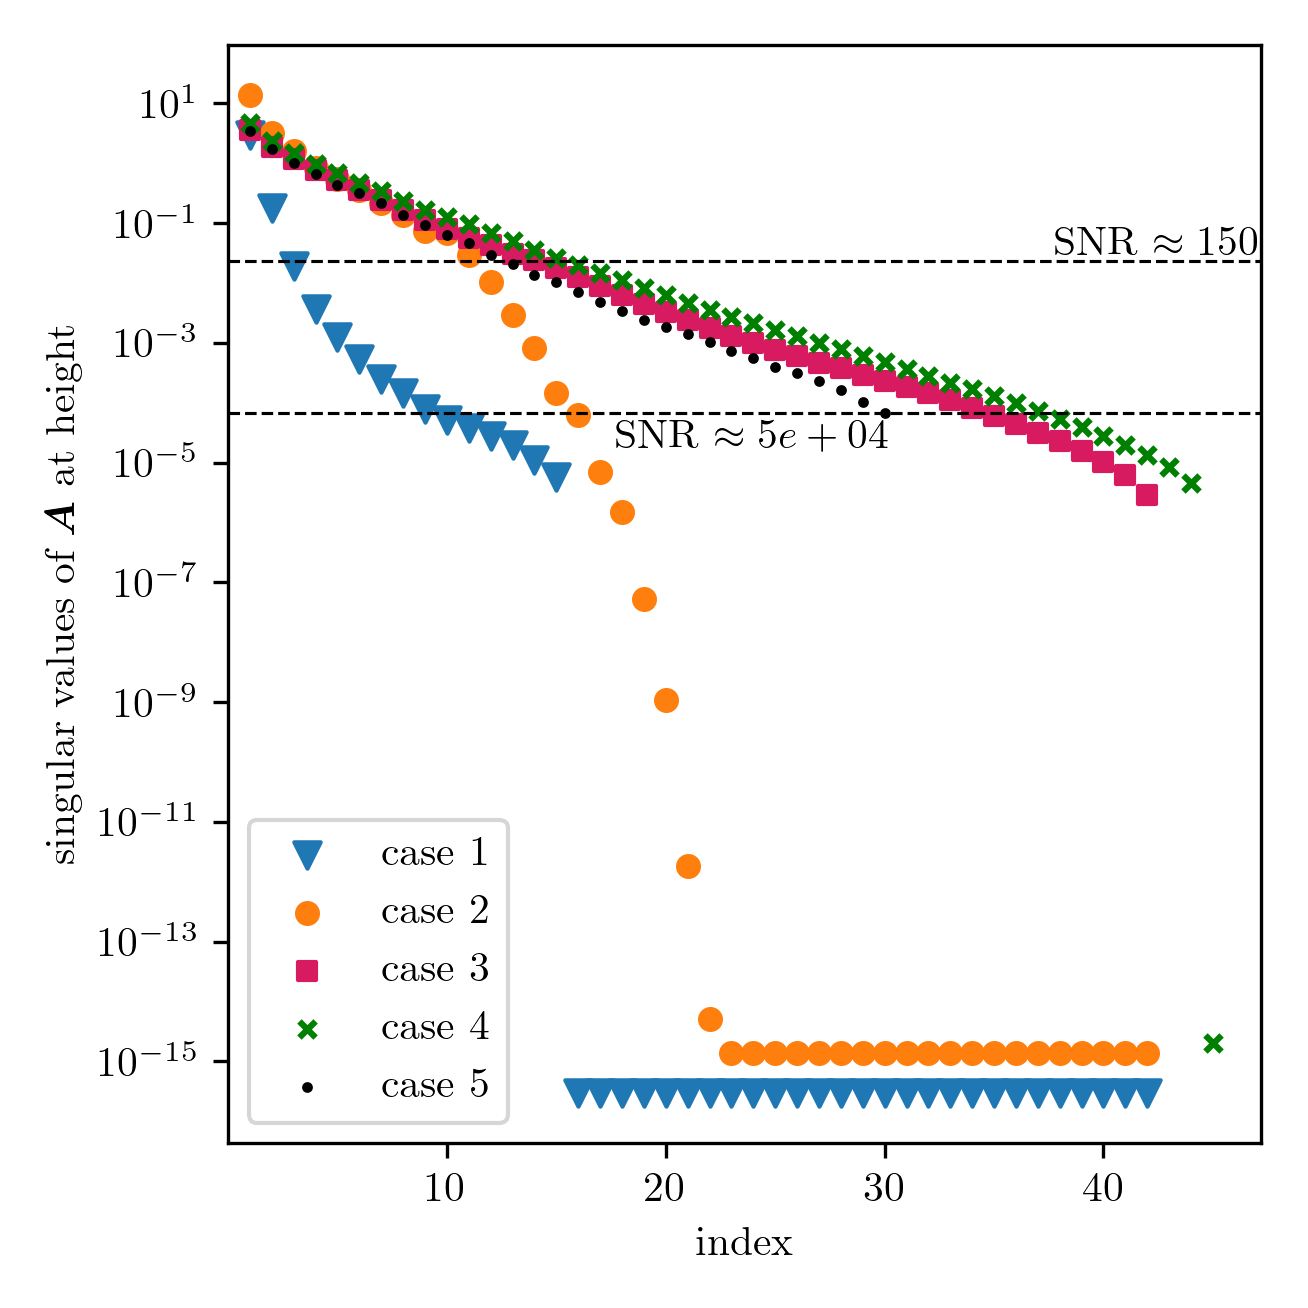
\includegraphics{SingValA.png}
	\caption[Singular values of linear forward model matrix for different sequences of measurements.]{Singular values of the forward model matrix for different sequences of measurements.
		The corresponding tangent heights of the test cases are plotted in Fig.~\ref{fig:TangHCases}. The dotted vertical line marks where the singular values are dominated by noise according to a specific SNR.}
	\label{fig:SingA}
\end{figure}
\textcolor{red}{oh no, I had hpped this section would be 'we' free.}
\textcolor{red}{where do you explain why this SNR has a line here?,
Were is the clear definition of these cases? I could not find it.}
Next, we plot the singular values for five different measurement scenarios, where we either measure at equidistance-spaced tangent heights or collect more data from high signal regions at low altitudes or from low signal regions at high altitudes.
We assess the number of singular values above and below a certain SNR visually to determine which of the tested cases is most effective. \textcolor{red}{Another, they are multiplying like rabbits. Or flies. Which is more annoying?}
We start with case 3 in Fig.~\ref{fig:TangHCases} where measurements are spaced according to a pointing accuracy of $150\text{arc sec}$, given to us by the team of the University of New South Wales Canberra Space~\cite{CubeSatInternal}. \textcolor{red}{more sentence creep. }
The pointing accuracy determines how well the satellite can point in a certain direction and, hence, roughly the spacing in between two measurements. \textcolor{red}{Actually, you should calculate this from the MIPAS specifications, or similar. It claims 1-3km resolution, presumably at a distance of 500km. So, what's that in arc seconds? It's also related to your vertical discretization, or, more to the point, your vertical discretization is determined by this.}
The corresponding singular values are plotted in Fig.~\ref{fig:SingA}, of which the first 25 decrease linearly in log-space and about 10-15 singular values lie above the SNR. \textcolor{red}{where is this spacing? At the satellite? A spacing in time? On the planet Mars. Be specific. All the way through, you need to tighten up loose statements like this.}
In comparison, if we measure a lot of times in regions where the data is noise-dominated (high altitude), case 1, we do obtain more information since the singular values decrease rapidly.
\textcolor{red}{Oh come on, you are showing pictures of singular values without specifying exactly what the forward map and discretization is. That's not acceptable. If these are intended to be indicative, you need to be a damn site clearer about what they represent, and are trying to show.}
Measuring lots of times at low altitudes, where the data is informative, and less at higher altitudes, case 2, does not seem optimal either, as we observe one larger singular value, but the other singular values decrease faster compared to case 3.
Now consider case 4, where we double the number of measurements compared to case 3, we do get slightly larger singular values, but not so significantly that it would be worth the engineering effort required to achieve that.
The measurements with equidistance-spaced tangent height seem to be most effective. \textcolor{red}{why? Explain your reasoning. If you don't say something specific, quantitative, it's just waffle.}
By exploratory analysis, we find that we can tolerate a slightly larger distance between tangent heights (pointing accuracy of $175\text{arc sec}$) than required by~\cite{CubeSatInternal}, see case 5.
In that case, we also stop measuring when the signal is too noisy and decrease the number of measurements taken without losing crucial information.
We note that if one wanted to obtain all information provided by the forward model, we would need a signal-to-noise ratio of roughly $10^7$.

In principle, we show that it does not depend on how one measures; one cannot get more information by measuring more in regions where the information content is low or high.
\textcolor{red}{on the contrary - -you have just been arguing that it does matter. no, this makes sense if the goal is to reduce noise.}
This contradicts the current measurement setup on the AURA MLS~\cite{livesey2006retrieval}, which reports high noise in lower atmospheric regions, due to thermal radiation from the earth, and measures more in those regions.

\begin{figure}[ht!]
	\centering
	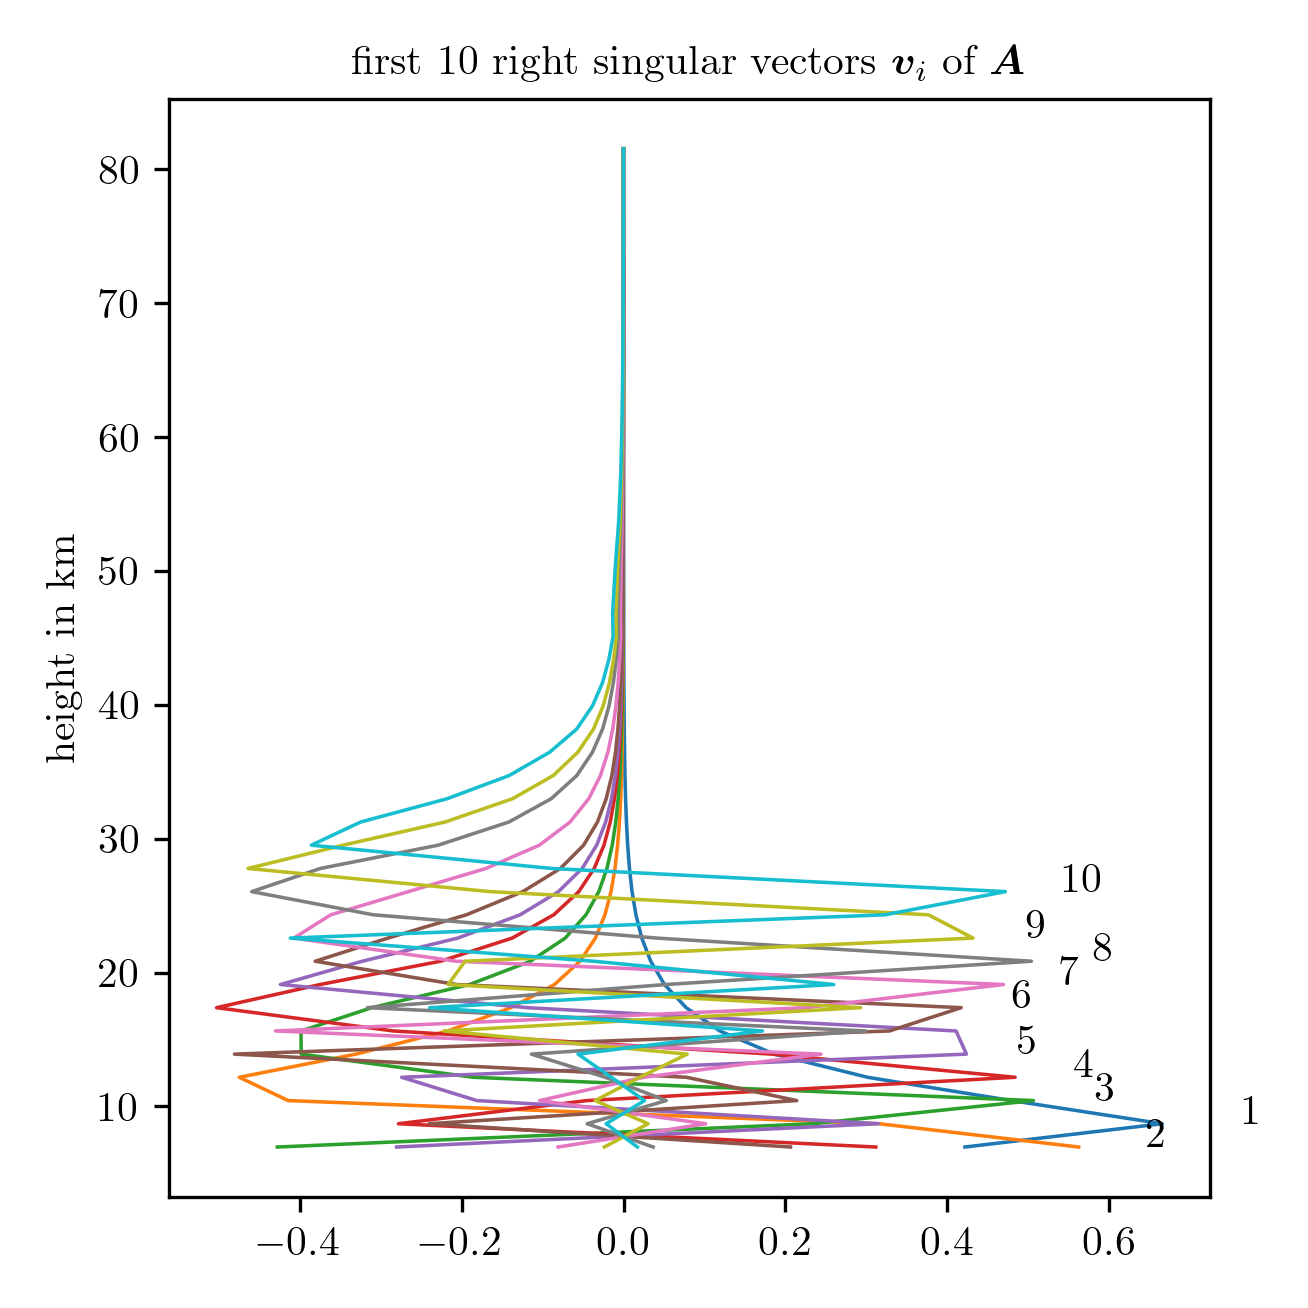
\includegraphics{SingVecA.png}
	\caption[First 10 right singular vectors of forward model.]{First 10 right singular vectors of the forward model matrix for measurements case 5 in Fig.~\ref{fig:TangHCases}. These singular vectors correspond to high singular values of the forward model in Fig.~\ref{fig:SingA}.}
	\label{fig:SingVecA}
\end{figure}
\begin{figure}[ht!]
	\centering
	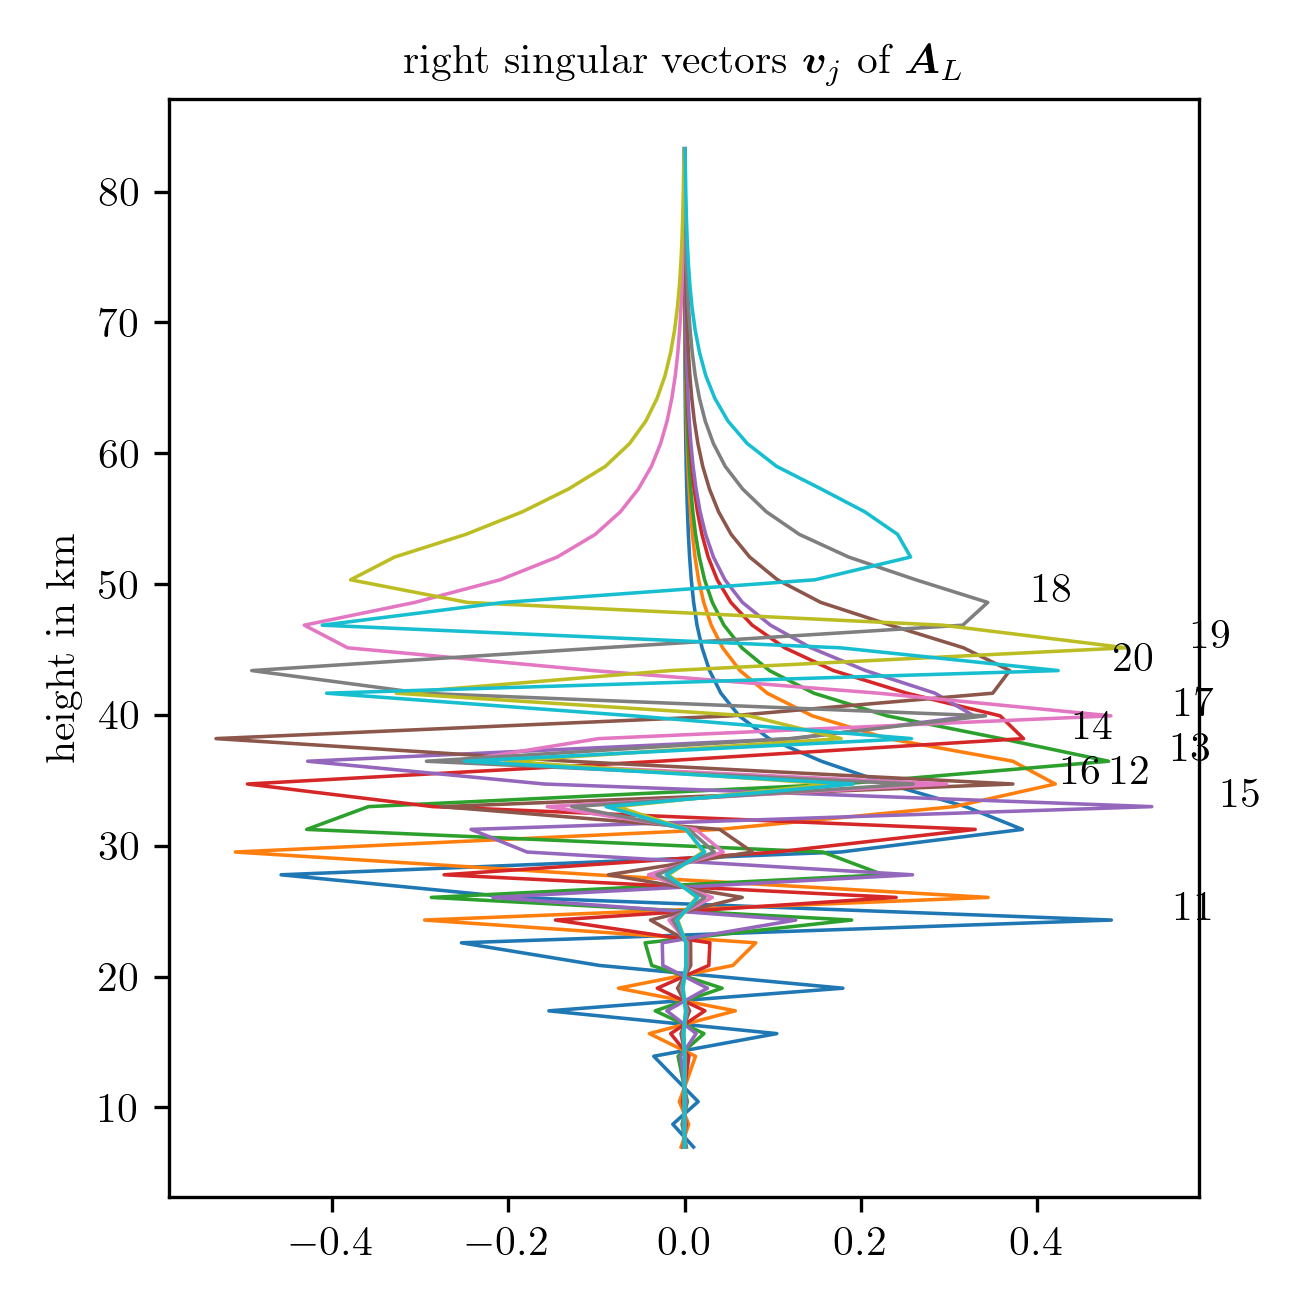
\includegraphics{MiddleVecA.png}
	\caption[Right singular vectors 11 to 19 of forward model.]{Right singular vectors with index $i = 11,\dots, 19$ of the forward model matrix for measurements case 5 in Fig.~\ref{fig:TangHCases}.
		These singular vectors correspond to singular values in Fig.~\ref{fig:SingA} where the noise level is similar to the data.}
	\label{fig:middleSpace}
\end{figure}
\begin{figure}[ht!]
	\centering
	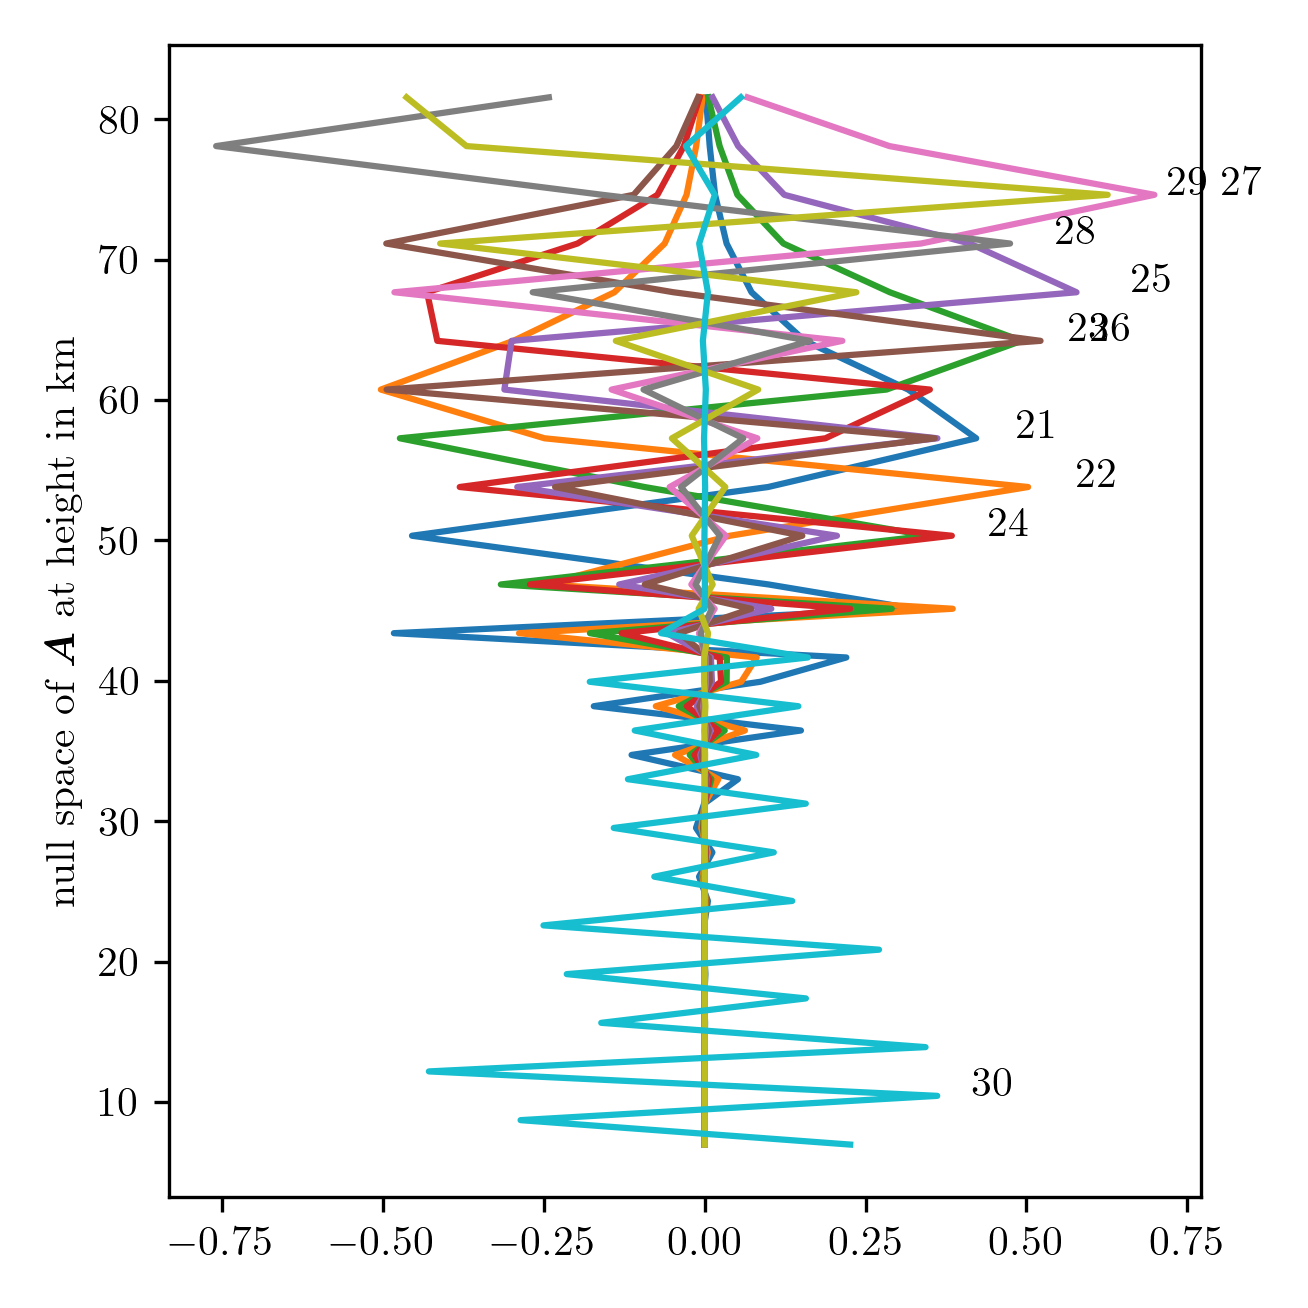
\includegraphics{NullVecA.png}
	\caption[Last 10 right singular vectors of forward model.]{Last 10 right singular vectors of the forward model matrix for measurements case 5 in Fig.~\ref{fig:TangHCases}. These singular vectors correspond to small singular values of the forward model in Fig.~\ref{fig:SingA} where the data is noise-dominated.}
	\label{fig:nullSpace}
\end{figure}

Consequently, we proceed with case 5 and plot the right singular vectors of the forward model versus height in the atmosphere to see where our model is most informative, or which structures of the parameter space are picked up by the model.
The first 10 right singular vectors, in Fig.~\ref{fig:SingVecA}, corresponding to the 10 largest singular values, pick up parameter structures in lower atmospheric regions.
So we can assume that, given some data, we will be able to provide good reconstructions of the parameter in lower altitudes. \textcolor{red}{too colloquial. One picks up rubbish, not sure what it means in this context.}
Next, we plot the right singular vectors corresponding to the singular values $\sigma_j$ for $j = 11, \dots, 20$ in Fig. \ref{fig:middleSpace}, where the noise starts to dominate the data.
These singular values lie in regions around the SNR, see Fig.~\ref{fig:SingA}, and pick up values in the middle of the atmosphere. \textcolor{red}{ditto}
Consequently, we expect a higher uncertainty of reconstructed parameter values in the middle atmospheric regions.
The singular vectors corresponding to the last 10 singular values pick up parameter structures in higher altitudes, but since the singular values are very small, we will not be able to retrieve those structures.
More specifically, the retrieved parameter values at higher altitudes will be mostly determined by the prior or, in the case of regularisation, by the regulariser~\cite{tan2016LecNot}.

